\chapter{Architettura del Sistema}
\label{capitolo4}
\thispagestyle{empty}

\begin{quotation}
{\footnotesize
\noindent \emph{}
\begin{flushright}
\end{flushright}
}
\end{quotation}
\vspace{0.5cm}

In questo capitolo descriveremo l'architettura del sistema implementato. Il sistema è stato progettato in maniera modulare per una serie di motivi: questo tipo di architettura permette di riutilizzare i moduli sviluppati, di estendere semplicemente il sistema con altri moduli, di sostituire eventualmente un intero modulo con un altro che compia le stesse funzioni, di comunicare in maniera semplice con altri sistemi. 

Per raggiungere qusto scopo, si è deciso quindi di utilizzare il middleware ROS (Robot Operating System)~\cite{quigley2009ros}.
ROS è un middleware che, oltre ad offrire molti tool utili per lo sviluppo di complesse applicazioni robotiche, implementa due pattern architetturali importanti, entrambi usati nel nostro lavoro: il pattern publish-subscribe e il pattern client-server.
Questi due patten sono implementati rispettivamente tramite messaggi e servizi: i messaggi definiscono un formato comune per la pubblicazione di dati in topic, i servizi invece specificano un'interfaccia per le chiamate a procedure remote, dichiarando gli input e gli output tra client e server.
Ogni processo che viene eseguito in ROS è chiamato nodo. Per eseguire qualsiasi sistema basato su ros, devono essere presenti tre ulteriori nodi: il nodo Master, che si occupa di garantire la comunicazione tra gli altri nodi, tramite i due pattern supportati, il server dei parametri, che implementa un dizionario condiviso accessibile tramite la rete, in cui i nodi posssono memorizzare e recuperare parametri usati dai loro algoritmi a runtime, il nodo rosout, che si occupa di mantenere i log prodotti dalle appliazioni.

Il sistema sviluppato è pensato per interagire con qualsiasi tipo di robot che sia provvisto di una videocamera monoculare e una unità di misura inerziale (IMU) tramite le due interfacce standard di ROS.
Esse consistono in tre topic: ``imu'', per i dati provenienti dall unità di misura inerziale, ``image\_raw'', per l'immagine proveniente dalla videocamera, ``camera\_info'', che contiene i parametri intrinseci della videocamera, tra cui la matrice di calibrazione della videocamera utilizzata, necessaria per il funzionamento del sistema.
I dati estratti dall'unità di misura inerziale devono essere riferiti al sistema di coordinate della videocamera, infatti l'algoritmo di visione implementato utilizza i dati provenienti dalla IMU per stimare approssimativamente la posa della telecamera.
%TODO sarebbe bello non avere questo vincolo, purchè sia nota la trasformazione dal sistema di coordinate della imu al sistema di coordinate della telecamera. Provo a implementarlo, dovrebbe essere semplice... c'è già il tpic di tf con le opportune trasformazioni...

\section{Diagramma del sistema}

L'architettura del sistema implementato è descritta in \autoref{fig:architettura-sistema}. \\
\begin{figure}[here]
  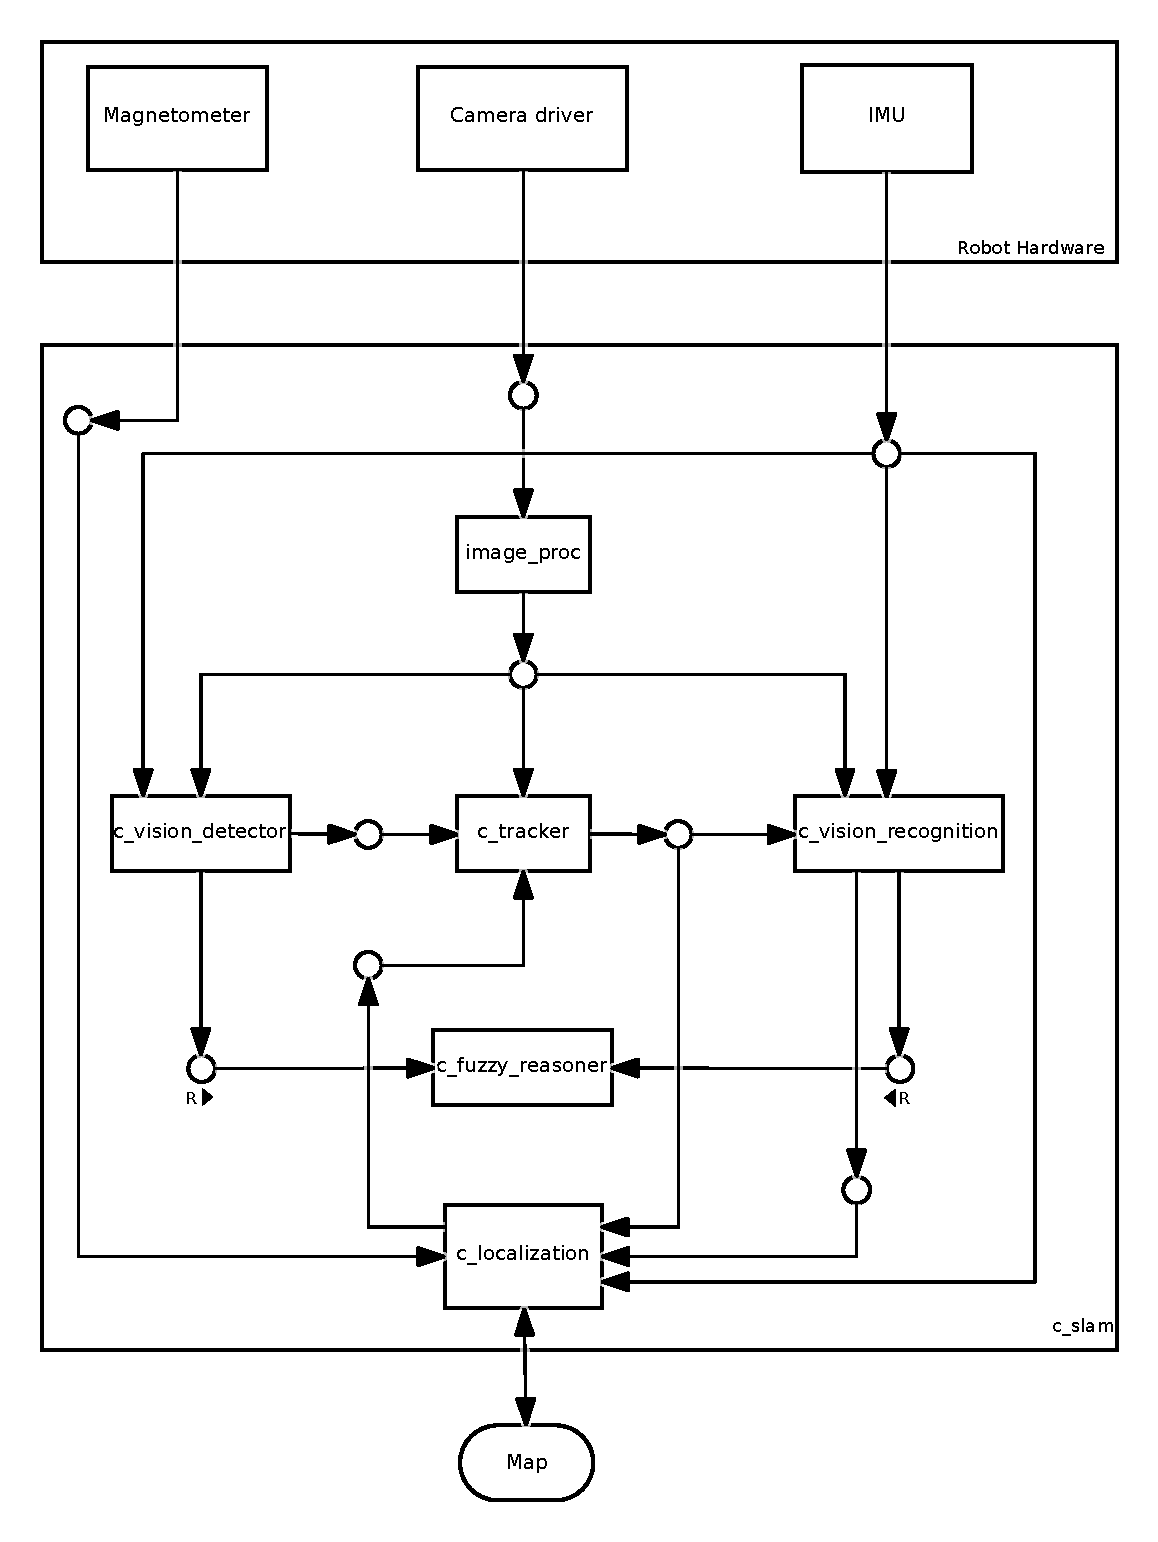
\includegraphics[width=0.9\textwidth]{diagrammi/Sistema}
  \caption{Architettura del sistema implementato}
  \label{fig:architettura-sistema}
\end{figure}


Il diagramma rappresenta i nodi del sistema, segue una breve descrizione di ogni elemento per specificare la loro funzione:

\begin{description}
  \item [image\_proc] si occupa di eliminare la distorsione radiale della videocamera causata dalla curvatura della lente.
  \item [c\_vision\_detector] si occupa di estrarre possibili feature dall'immagine.
  \item [c\_tracking] si occupa di seguire le feture a basso livello estratte dal nodo ``c\_vision\_detector'' nell'immagine, mantenendo un modello in modo da riuscire a riconoscere la feature anche dopo essere stata persa. 
  \item [c\_vision\_slam] si occupa dell'analisi approfondita delle feature, in modo da determinare il tipo di oggetto e la sua posizione nello spazio. 
  \item [c\_fuzzy\_reasoner] implementa un reasoner fuzzy; data una base di conoscenza e un classificatore, analizza le feature in ingresso e le classifica. 
\end{description}



